\section{表观遗传学}
\subsection{概述}
\begin{frame}
  \frametitle{表观遗传学 | 简介}
  \begin{figure}
    \centering
    
\includegraphics[width=0.6\textwidth]{c3.transcriptome/epi.intro.06.jpg}
    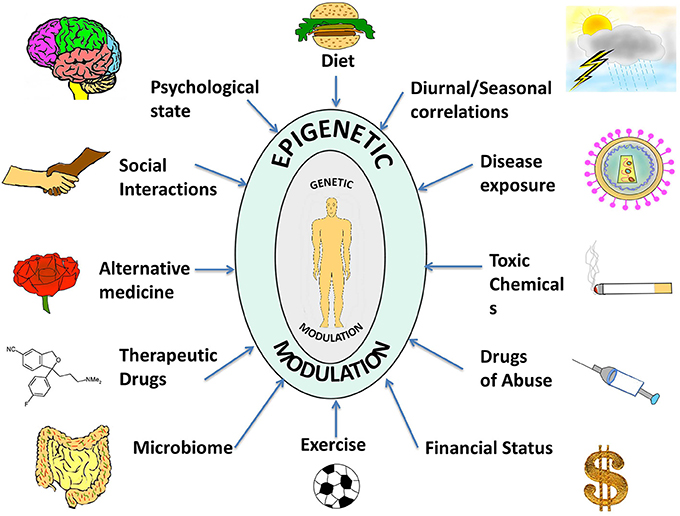
\includegraphics[width=0.4\textwidth]{c3.transcriptome/epi.intro.04.jpg}
  \end{figure}
\end{frame}

\begin{frame}
  \frametitle{表观遗传学 | \textcolor{red}{简介}}
  \begin{block}{表观遗传学}
表观遗传学(epigenetics)研究的是在不改变DNA序列的前提下,通过某些机制引起可遗传的基因表达或细胞表现型的变化。 表观遗传学是20世纪80年代逐渐兴起的一门学科,是在研究与经典的孟德尔遗传学遗传法则不相符的许多生命现象过程中逐步发展起来的。\\
\vspace{1em}
表观遗传现象包括DNA甲基化、组蛋白修饰、RNA干扰等。与经典遗传学以研究基因序列影响生物学功能为核心相比,表观遗传学主要研究这些“表观遗传现象”建立和维持的机制。其研究内容主要包括两类,一类为基因选择性转录表达的调控,有DNA甲基化、基因印记、组蛋白共价修饰和染色质重塑;另一类为基因转录后的调控,包括基因组中非编码RNA、微小RNA、反义RNA、内含子及核糖开关等。\\
\vspace{1em}
表观遗传学指基因组相关功能改变而不涉及核苷酸序列变化,即“由染色体改变所引起的稳定的可遗传的表现型,而非DNA序列的改变”。
  \end{block}
\end{frame}

\begin{frame}
  \frametitle{表观遗传学 | 简介}
  \begin{figure}
    \centering
    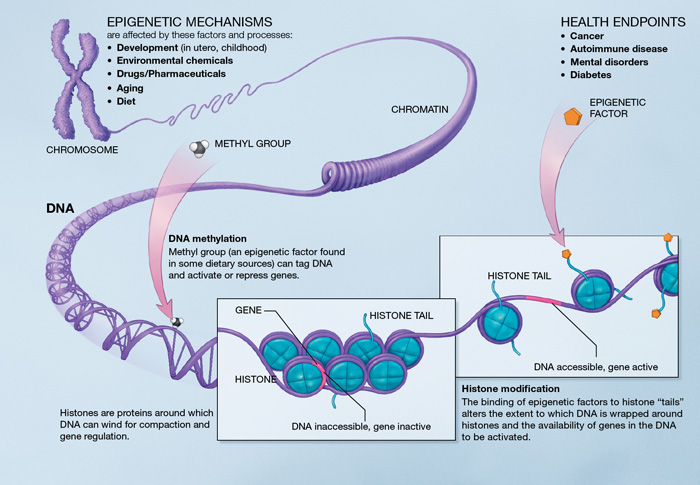
\includegraphics[width=0.9\textwidth]{c3.transcriptome/epi.intro.01.jpg}
  \end{figure}
\end{frame}

\begin{frame}
  \frametitle{表观遗传学 | \textcolor{red}{简介}}
  \begin{figure}
    \centering
    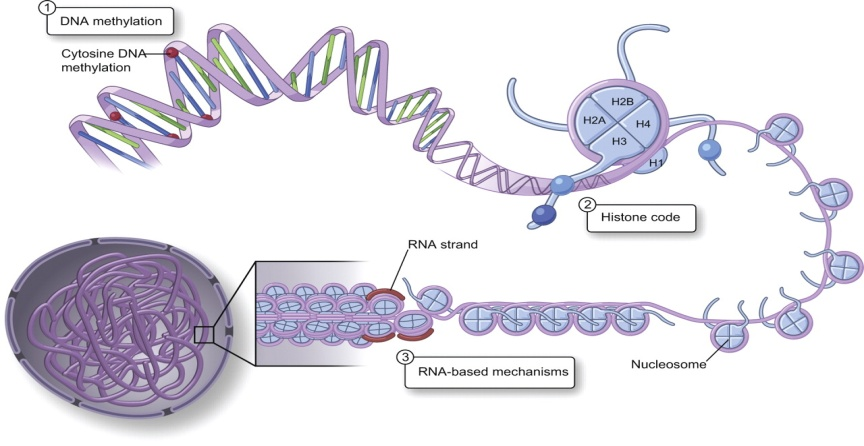
\includegraphics[width=0.9\textwidth]{c3.transcriptome/epi.intro.02.jpg}
  \end{figure}
\end{frame}

\begin{frame}
  \frametitle{表观遗传学 | \textcolor{red}{DNA甲基化}}
  \begin{block}{DNA甲基化}
    DNA甲基化(DNA methylation)为DNA化学修饰的一种形式,能在不改变DNA序列的前提下,改变遗传表现。为外遗传编码(epigenetic code)的一部分,是一种外遗传机制。DNA甲基化过程会使甲基添加到DNA分子上,例如在胞嘧啶环的5'碳上:这种5'方向的DNA甲基化方式可见于所有脊椎动物。 特定胞嘧碇受甲基化的情形,可利用亚硫酸盐测序(bisulfite sequencing)方式测定。DNA甲基化可能使基因沉默化,进而使其失去功能。\\
    \vspace{0.5em}
    在人类细胞内,大约有1\%的DNA碱基受到了甲基化。在成熟体细胞组织中,DNA甲基化一般发生于CpG双核苷酸(CpG dinucleotide)部位;而非CpG甲基化则在胚胎干细胞中较为常见。\\
    \vspace{0.5em}
    植物体内胞嘧啶的甲基化则可分为对称的CpG(或CpNpG),或是不对称的CpNpNp形式(C与G是碱基;p是磷酸根;N指的是任意的核苷酸)。
  \end{block}
\end{frame}

\begin{frame}
  \frametitle{表观遗传学 | DNA甲基化}
  \begin{block}{DNA甲基化与肿瘤}
 DNA甲基化是一种基因转录的重要的调节器,许多证据已经证实,异常的DNA甲基化与不定期的基因沉默有关,若在启动子区域具有高水平的5-甲基胞嘧啶,将发生基因沉默。\\
 \vspace{0.5em}
DNA甲基化在胚胎发育期间是必需的,在体细胞中,DNA甲基化的方式通常是高保真的传给子细胞。\\
 \vspace{0.5em}
异常的DNA甲基化模式与大量的人类恶性肿瘤有关,并发现其与正常组织相比存在两种不寻常的形式:超甲基化和低甲基化。超甲基化是主要的表观遗传修饰中的一种,其通过肿瘤抑制基因的启动子区抑制转录。超甲基化通常发生在启动子区的CpG岛,且与基因失活有关。整体的低甲基化也通过不同机制与癌症的发生和发展有关。 
  \end{block}
\end{frame}

\begin{frame}
  \frametitle{表观遗传学 | \textcolor{red}{DNA甲基化}}
  \begin{figure}
    \centering
    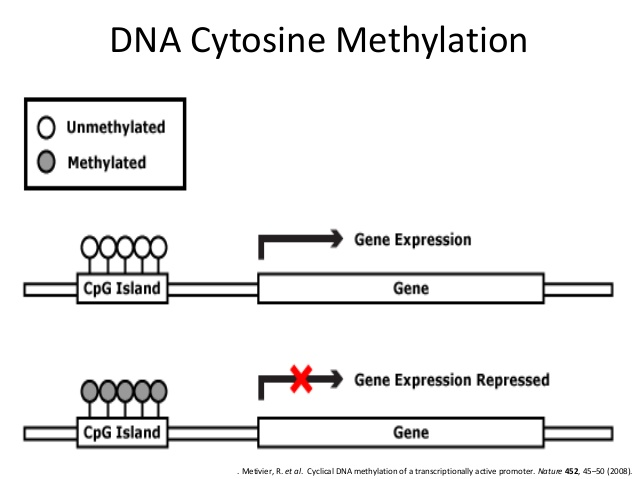
\includegraphics[width=0.8\textwidth]{c3.transcriptome/epi.methy.01.jpg}
  \end{figure}
\end{frame}

\subsection{Methyl-Seq}
\subsubsection{数据分析}
\begin{frame}
  \frametitle{表观遗传学 | Methyl-Seq | 分析 | 流程}
  \begin{figure}
    \centering
    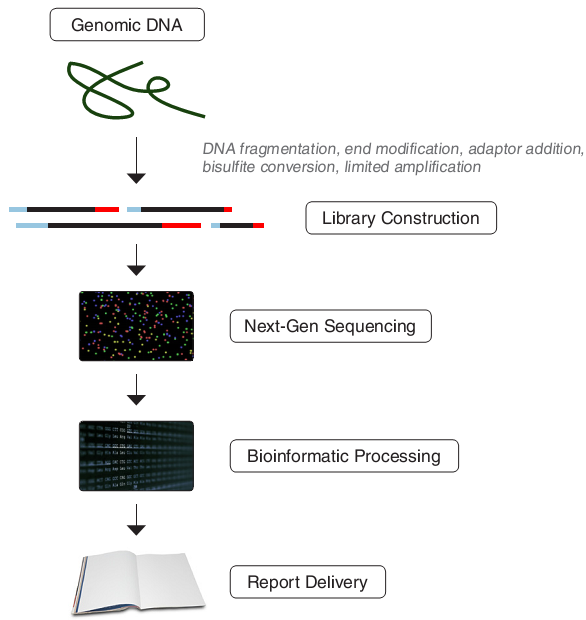
\includegraphics[width=0.6\textwidth]{c3.transcriptome/mseq.all.01.png}
  \end{figure}
\end{frame}

\begin{frame}
  \frametitle{表观遗传学 | Methyl-Seq | 分析 | 流程 | \textcolor{red}{实验}}
  \begin{figure}
    \centering
    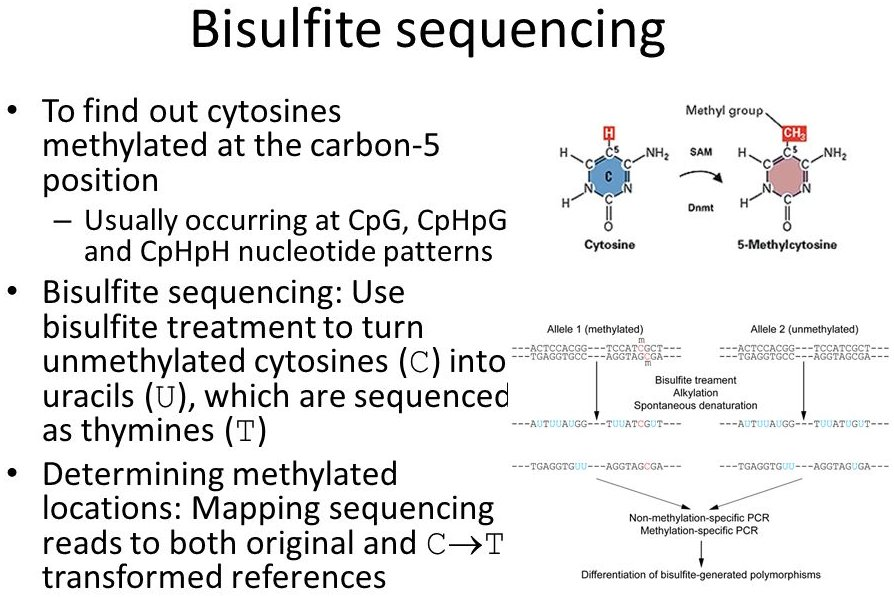
\includegraphics[width=0.9\textwidth]{c3.transcriptome/mseq.exp.00.jpg}
  \end{figure}
\end{frame}

\begin{frame}
  \frametitle{表观遗传学 | Methyl-Seq | 分析 | 流程 | \textcolor{red}{实验}}
  \begin{figure}
    \centering
    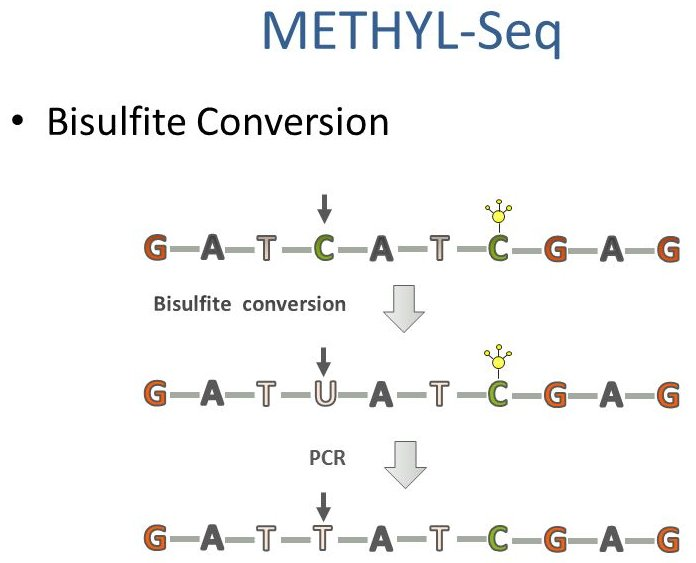
\includegraphics[width=0.4\textwidth]{c3.transcriptome/mseq.exp.01.jpg}\\
    \vspace{1em}
    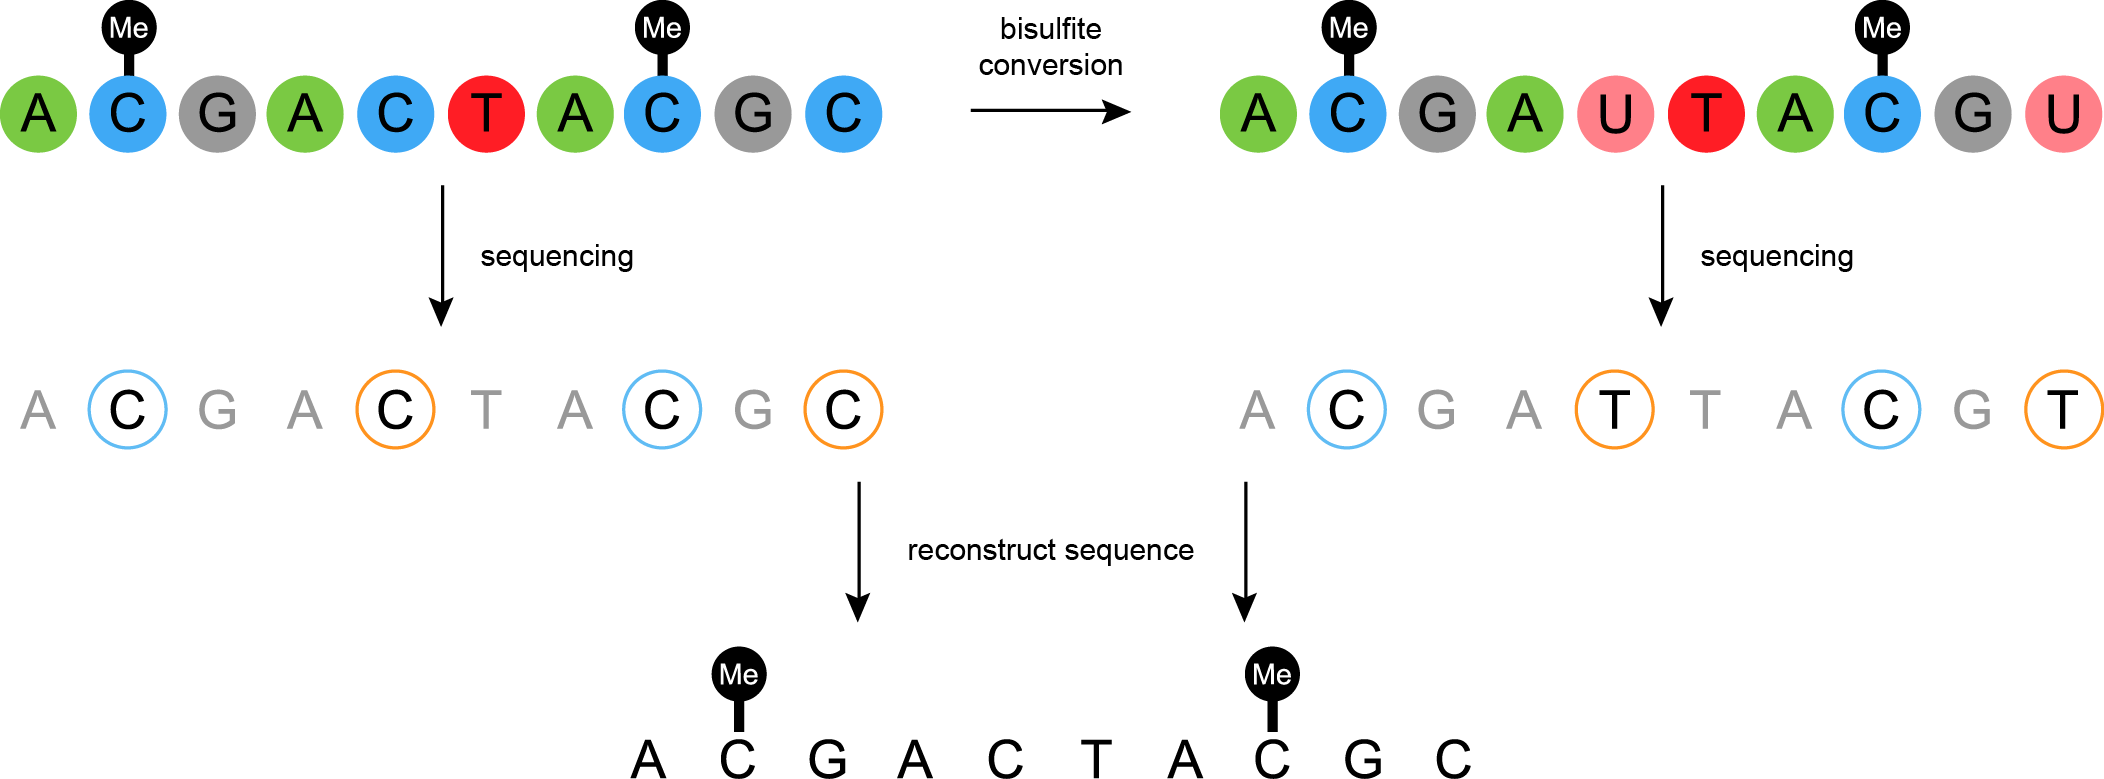
\includegraphics[width=0.6\textwidth]{c3.transcriptome/mseq.exp.03.png}
  \end{figure}
\end{frame}

\begin{frame}
  \frametitle{表观遗传学 | Methyl-Seq | 分析 | 流程 | 实验}
  \begin{figure}
    \centering
    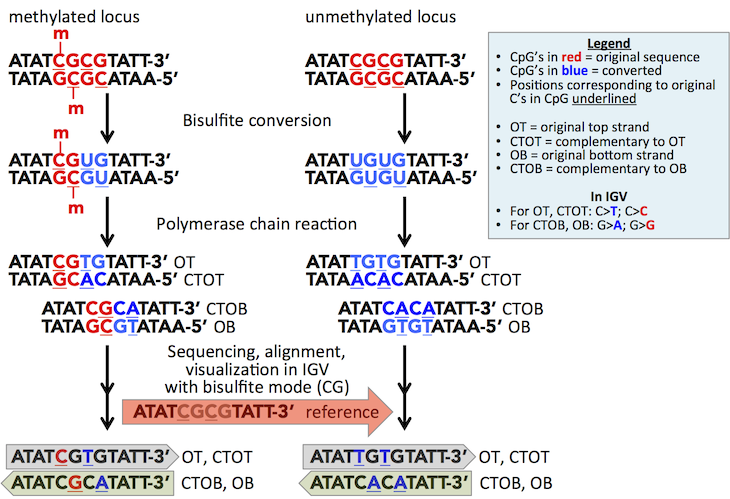
\includegraphics[width=0.9\textwidth]{c3.transcriptome/mseq.exp.04.png}
  \end{figure}
\end{frame}

\begin{frame}
  \frametitle{表观遗传学 | Methyl-Seq | 分析 | 流程 | 实验}
  \begin{figure}
    \centering
    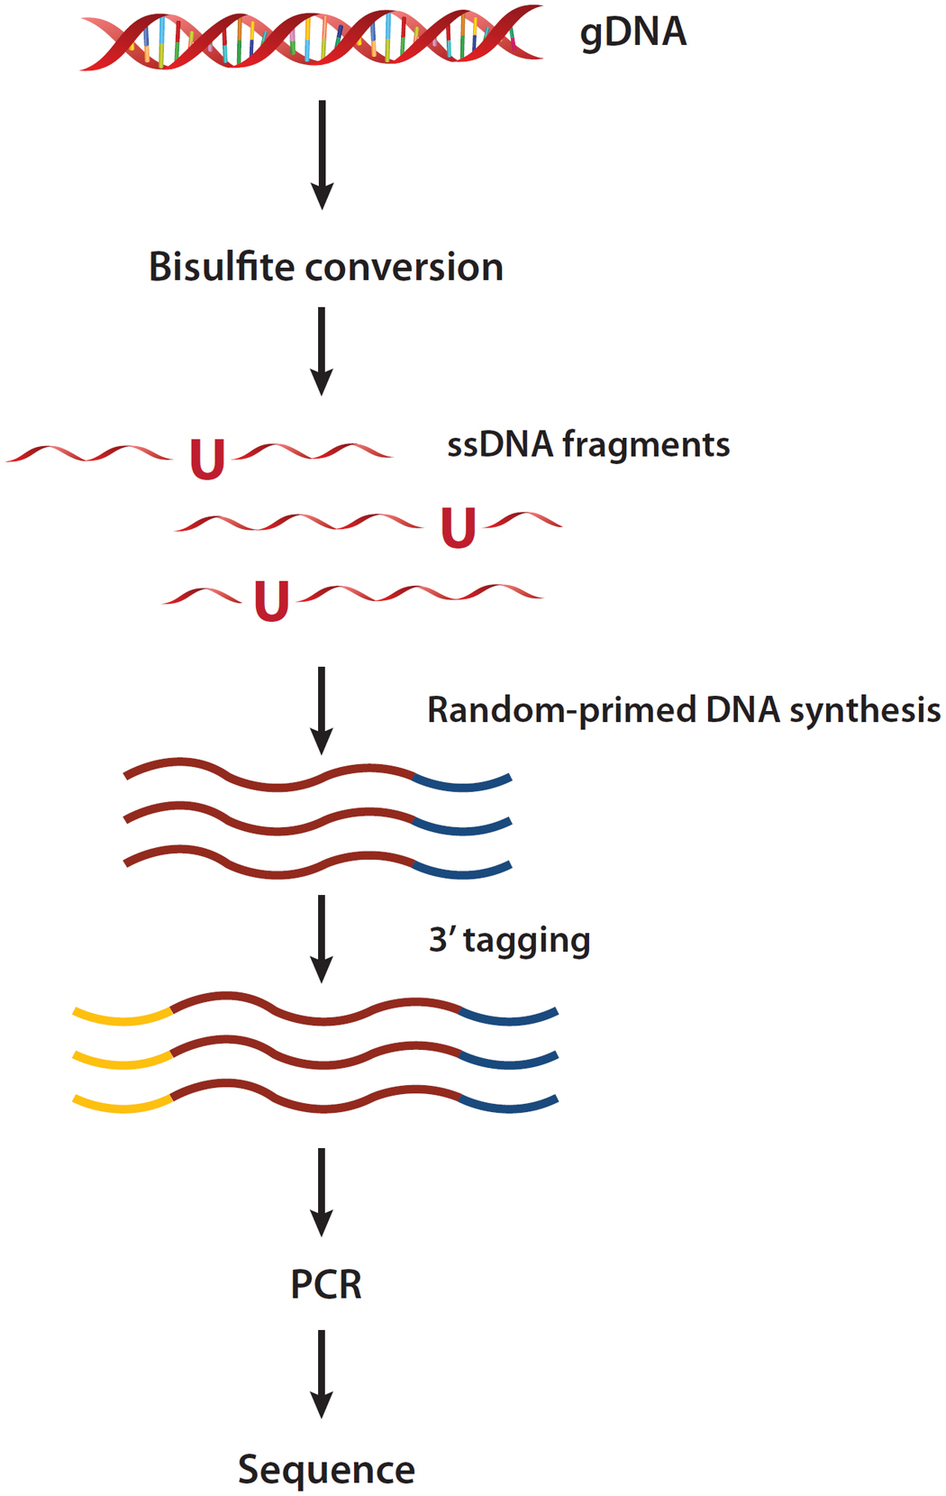
\includegraphics[width=0.4\textwidth]{c3.transcriptome/mseq.exp.02.jpg}
  \end{figure}
\end{frame}

\begin{frame}
  \frametitle{表观遗传学 | Methyl-Seq | 分析 | 流程 | 生信}
  \begin{figure}
    \centering
    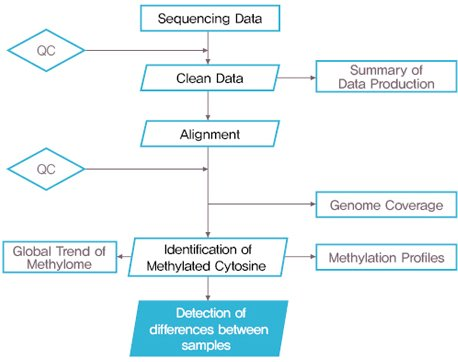
\includegraphics[width=0.8\textwidth]{c3.transcriptome/mseq.bx.01.jpg}
  \end{figure}
\end{frame}

\begin{frame}
  \frametitle{表观遗传学 | Methyl-Seq | 分析 | 流程 | \textcolor{red}{生信}}
  \begin{figure}
    \centering
    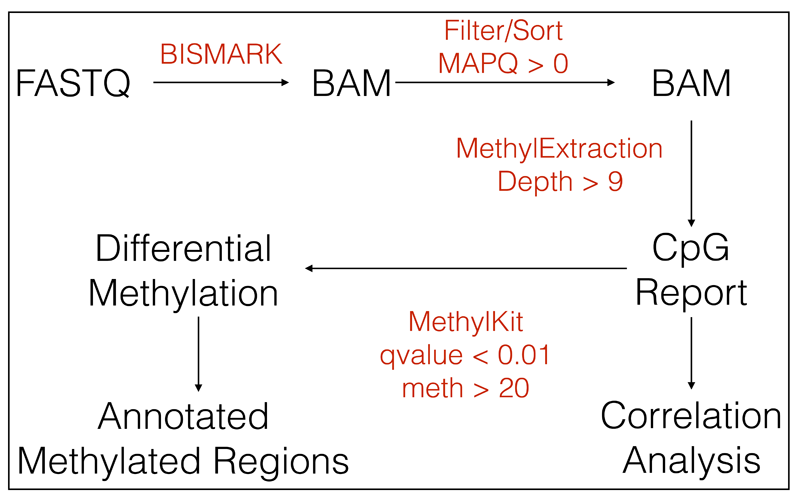
\includegraphics[width=0.9\textwidth]{c3.transcriptome/mseq.bx.02.png}
  \end{figure}
\end{frame}

\begin{frame}
  \frametitle{表观遗传学 | Methyl-Seq | 分析 | 流程 | 生信}
  \begin{figure}
    \centering
    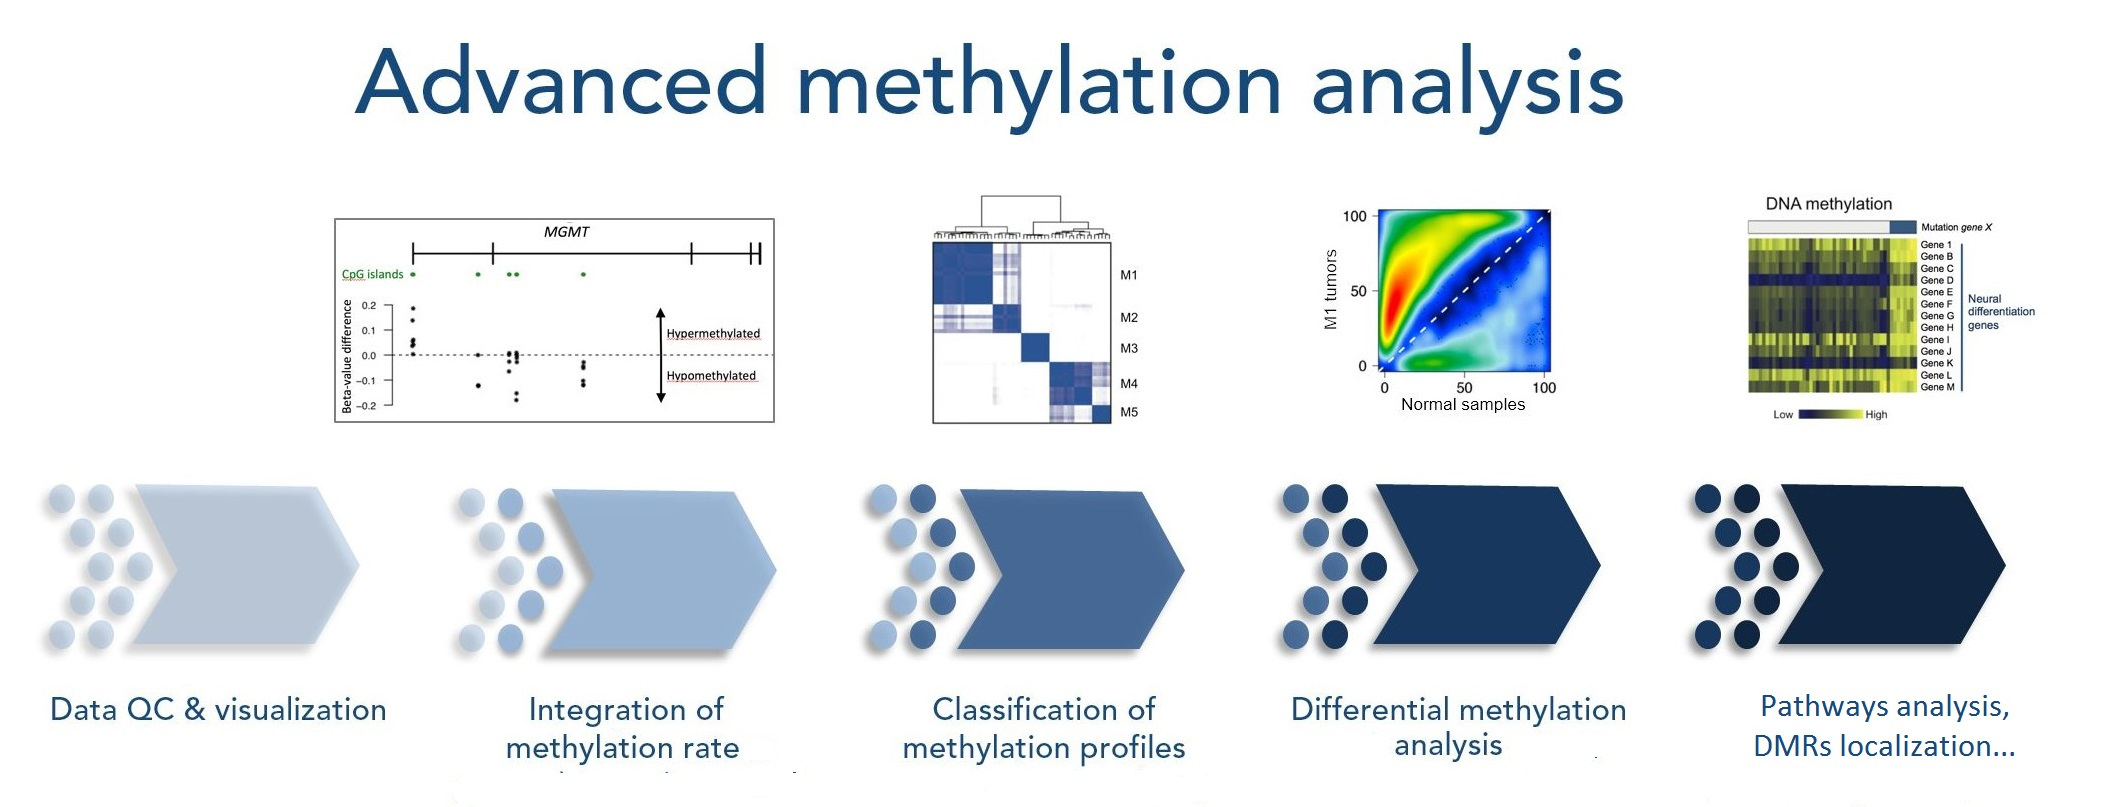
\includegraphics[width=0.9\textwidth]{c3.transcriptome/mseq.bx.03.jpg}
  \end{figure}
\end{frame}

\begin{frame}
  \frametitle{表观遗传学 | Methyl-Seq | 分析 | 流程 | 生信}
  \begin{figure}
    \centering
    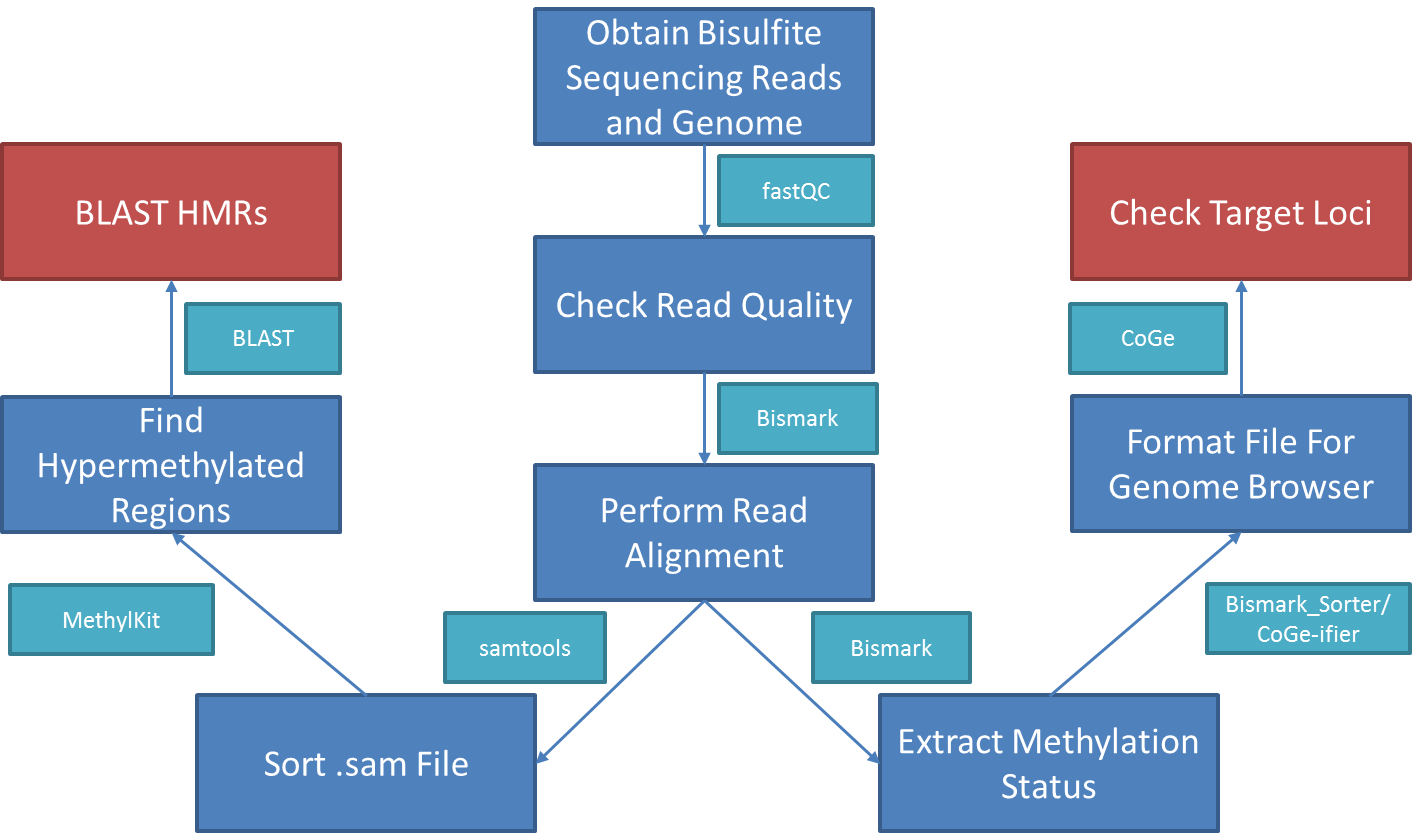
\includegraphics[width=0.9\textwidth]{c3.transcriptome/mseq.bx.04.png}
  \end{figure}
\end{frame}

\begin{frame}
  \frametitle{表观遗传学 | Methyl-Seq | 分析 | 流程 | 生信}
  \begin{figure}
    \centering
    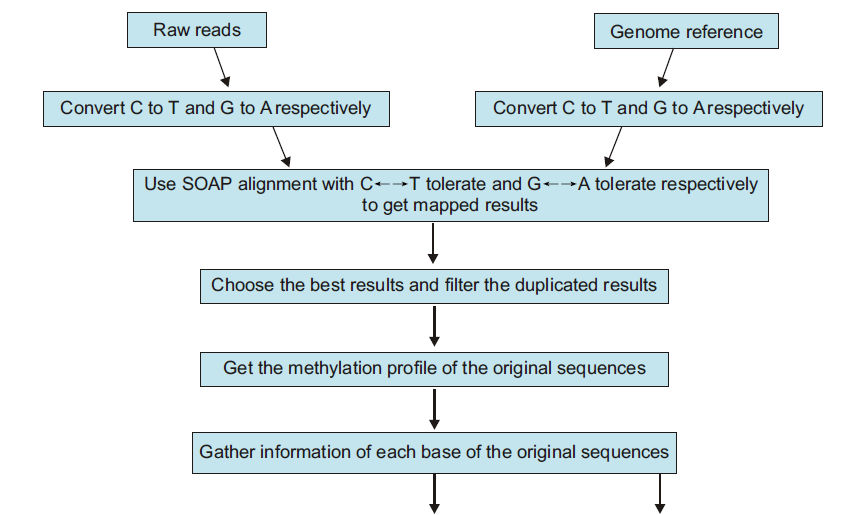
\includegraphics[width=0.58\textwidth]{c3.transcriptome/mseq.bx.05.png}\\
    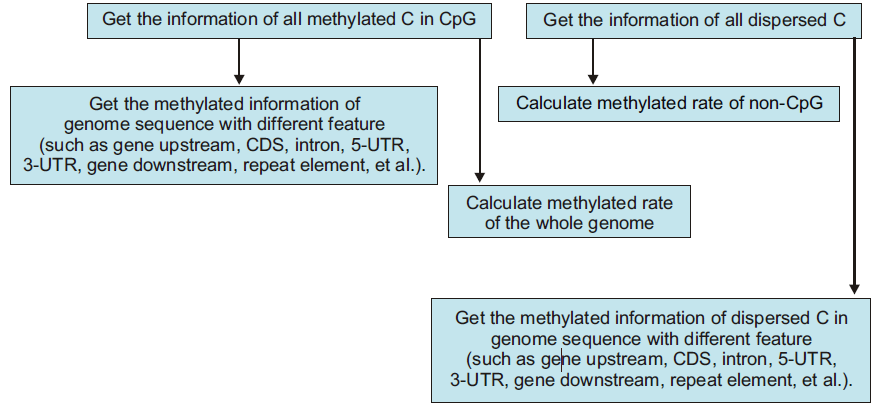
\includegraphics[width=0.58\textwidth]{c3.transcriptome/mseq.bx.06.png}
  \end{figure}
\end{frame}

\begin{frame}
  \frametitle{表观遗传学 | Methyl-Seq | 分析 | 流程 | 生信}
  \begin{figure}
    \centering
    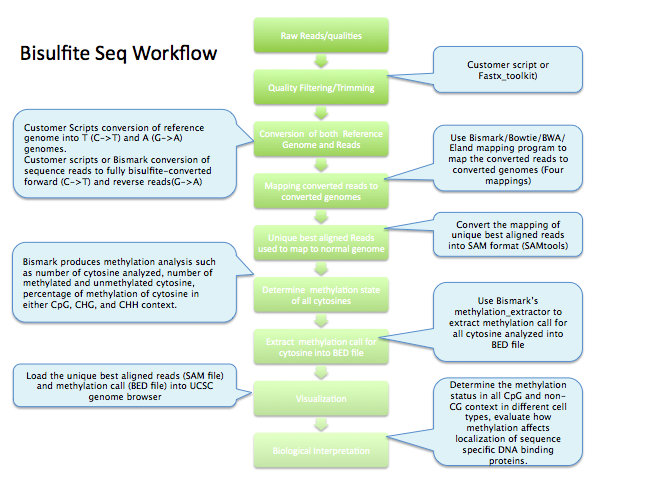
\includegraphics[width=0.85\textwidth]{c3.transcriptome/mseq.bx.07.png}
  \end{figure}
\end{frame}

\begin{frame}
  \frametitle{表观遗传学 | Methyl-Seq | 分析 | 流程 | \textcolor{red}{生信}}
  \begin{figure}
    \centering
    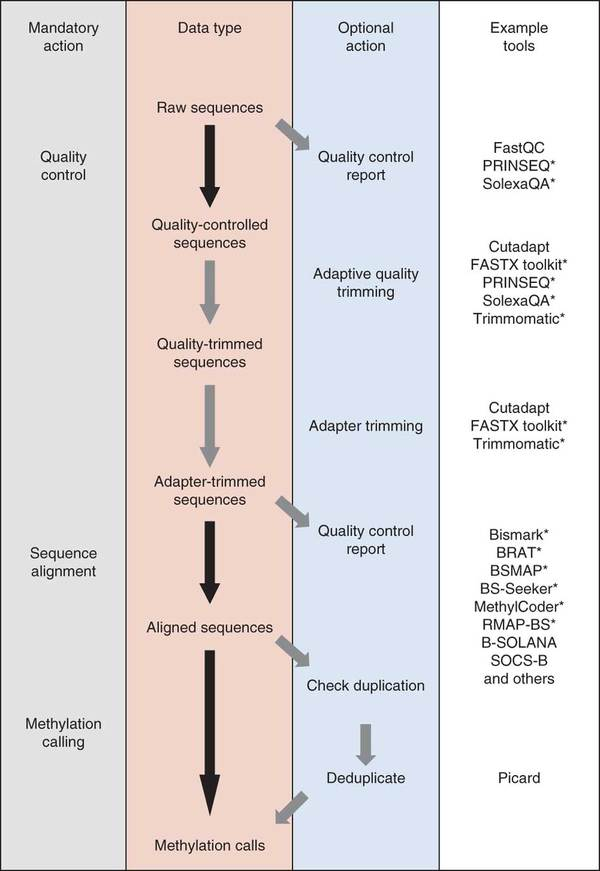
\includegraphics[width=0.45\textwidth]{c3.transcriptome/mseq.bx.08.jpg}
  \end{figure}
\end{frame}

\begin{frame}
  \frametitle{表观遗传学 | Methyl-Seq | 分析 | 应用}
  \begin{figure}
    \centering
    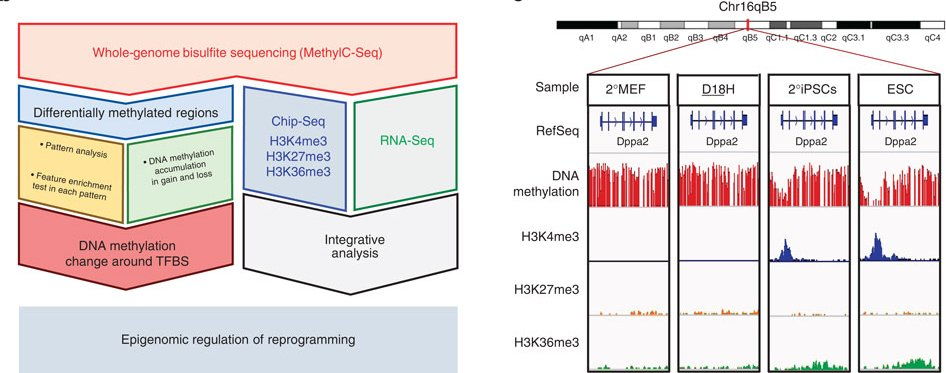
\includegraphics[width=0.9\textwidth]{c3.transcriptome/mseq.seqs.01.jpg}
  \end{figure}
\end{frame}

\begin{frame}
  \frametitle{表观遗传学 | Methyl-Seq | 分析 | \textcolor{red}{工具}}
  {\footnotesize
  \begin{block}{Bismark}
    Bismark is a program to map bisulfite treated sequencing reads to a genome of interest and perform methylation calls in a single step. The output can be easily imported into a genome viewer, such as SeqMonk, and enables a researcher to analyse the methylation levels of their samples straight away.
  \end{block}
  \pause
  \begin{block}{bwa-meth}
  Fast and accurante alignment of BS-Seq reads.
  \end{block}
  \pause
  \begin{block}{methylKit}
    methylKit is an R package for DNA methylation analysis and annotation from high-throughput bisulfite sequencing. The package is designed to deal with sequencing data from RRBS and its variants, but also target-capture methods such as Agilent SureSelect methyl-seq. In addition, methylKit can deal with base-pair resolution data for 5hmC obtained from Tab-seq or oxBS-seq. It can also handle whole-genome bisulfite sequencing data if proper input format is provided.
  \end{block}
  }
\end{frame}

\subsubsection{应用实例}
\begin{frame}
  \frametitle{表观遗传学 | Methyl-Seq | 实例}
  \begin{block}{Genome Research, 2009}
    To investigate the role of DNA methylation during human development, we developed Methyl-seq, a method that assays DNA methylation at more than 90,000 regions throughout the genome. Performing Methyl-seq on human embryonic stem cells (hESCs), their derivatives, and human tissues allowed us to identify several trends during hESC and in vivo liver differentiation. Taken together, our results indicate that hESC differentiation has a unique DNA methylation signature that may not be indicative of \textit{in vivo} differentiation.\\
    \vspace{0.5em}
    Brunner AL, Johnson DS, Kim SW, Valouev A, Reddy TE, Neff NF, et al. Distinct DNA methylation patterns characterize differentiated human embryonic stem cells and developing human fetal liver. Genome Res. 2009;19: 1044–1056.
  \end{block}
\end{frame}

\begin{frame}
  \frametitle{表观遗传学 | Methyl-Seq | 实例}
  \begin{figure}
    \centering
    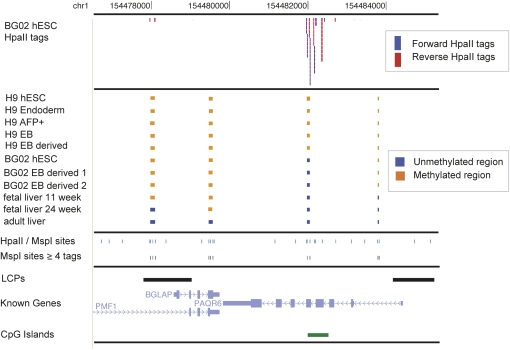
\includegraphics[width=0.9\textwidth]{c3.transcriptome/metseq.example.01.jpg}
  \end{figure}
\end{frame}

